\chapter{Conjuntos ordenados}

Una vez establecidos los conceptos necesarios, se introducen a continuación los 
\textbf{conjuntos ordenados}. El propósito de este capítulo es explicar cómo estos 
conjuntos almacenan a los multi-intervalos, presentar las distintas optimizaciones que se 
obtuvieron para estos, denominadas \textit{criterios de optimización} y \textit{criterios de ordenamiento} y, finalmente, detallar cómo dichas 
optimizaciones fueron incorporadas en las operaciones de los conjuntos ordenados.


\section{Estructura y orden}

Como se mencionó previamente en la sub-sección dedicada a los conjuntos ordenados densos, estos utilizaban el operador $<$ definido para los multi-intervalos para dotarse de orden. Los \textbf{conjuntos ordenados} utilizan el mismo criterio. Por lo tanto, la estructura de los conjuntos ordenados, denominados \texttt{OrderedSet}, incluye la siguiente variable miembro:

\begin{itemize}
  \item \texttt{pieces\_} (de tipo \textbf{MDIOrdSet}): Representa el conjunto en sí mismo.
\end{itemize}

Ahora bien, a diferencia de los conjuntos ordenados densos, que operaban sobre una única dimensión, los conjuntos ordenados trabajan sobre múltiples dimensiones. En consecuencia, el operador $<$ definido para el tipo \texttt{MD\_NAT} ya no se limita a una comparación tradicional entre valores numéricos, sino que ya trabaja a nivel dimensional como se mostró en la Sub-sección~\ref{sec:conjs-ord-dense}.

Supóngase que se trabaja con multi-intervalos bidimensionales, donde cada uno posee su correspondiente mínimo. Sean entonces por ejemplo los siguientes tres multi-intervalos:

\begin{itemize}
    \item $mdi_1 =$ $[2:1:2]\times[3:2:9]$, con mínimo $(2,\ 3)$
    \item $mdi_2 =$ $[1:1:2]\times[5:2:9]$, con mínimo $(1,\ 5)$
    \item $mdi_3 =$ $[2:1:2]\times[1:2:9]$, con mínimo $(2,\ 1)$
\end{itemize}

Aplicando el criterio de orden basado en los mínimos, con el operador $<$ definido para los multi-intervalos, se obtiene el siguiente ordenamiento:

\begin{center}
\[
mdi_2 < mdi_3 < mdi_1
\]

ya que:

\[
(1,\ 5) < (2,\ 1) < (2,\ 3)
\]

Por lo tanto, el conjunto ordenado resultante será:

\[
\{mdi_2,\ mdi_3,\ mdi_1\}
\]
\end{center}

\section{\textit{Abstarct factory}}

Al igual que se hizo con los conjuntos desordenados y ordenados densos,
también se definió la fábrica concreta para los conjuntos ordenados, para poder aplicar el patrón \textit{Abstarct factory}. 

En particular, la fábrica concreta de los conjuntos ordenados se denominó 
\texttt{OrdAF}. Esta puede encontrarse en los archivos 
\textit{af\_set}, tanto en su versión 
\textit{.cpp} como \textit{.hpp}, dentro de la carpeta \texttt{sbg} del repositorio.

\section{Criterios de optimización y ordenamiento}\label{sec:opts}

En esta sección se describen en detalle los diferentes \textbf{criterios de optimización}, así como los \textbf{criterios de ordenamiento} empleados en las operaciones para conjuntos ordenados. Ambos conjuntos de criterios se aplicarán posteriormente con el objetivo de mejorar la eficiencia general de las operaciones y reducir significativamente los tiempos de ejecución.

Ahora bien, para que todo este claro, un \textit{criterio de optimización} es, en esencia, un predicado que permite mejorar el rendimiento de una operación, aprovechando una o varias propiedades de una estructura de datos y de los elementos que esta contiene. Mientras un \textit{criterio de ordenamiento} es una regla que define cómo organizar de manera eficiente los elementos dentro de una estructura de datos para que se cumpla un cierto orden.


\textbf{Pseudocódigo y notación:} A partir de este momento, en este capítulo, al igual que se hizo para los conjuntos desordenados, se emplearán subíndices para referirse a los multi-intervalos de un conjunto ordenado. Dado un conjunto ordenado $A$, el elemento ubicado en la posición $i$, lo cual corresponde a \texttt{pieces\_[i]} en C++, se denotará como \textbf{$A_i$}, donde $i$ es un número natural que satisface $0 \leq i < \kappa(A)$, siendo $\kappa(A)$ la aridad del conjunto $A$, es decir, la cantidad total de elementos que contiene. Cabe destacar que, al tratarse de un conjunto ordenado, siempre se cumple que $A_i < A_j$ si y sólo si $i < j$, para todo par de $i$ y $j$ tal que $0  \leq i, j < \kappa(A)$. Adicionalmente se dirá que, en el caso anterior, $A_i$ está \textbf{antes} de $A_j$ en $A$, mientras $A_j$ está \textbf{después} de $A_i$. Toda esta notación, adicionalmente, se puede encontrar dentro del \textbf{Apéndice~A}.

\subsection{Intersección - \texttt{intersection}}\label{sec:opts-int}

La operación \texttt{intersection} constituye un componente central dentro de la batería de operaciones fundamentales para conjuntos. Antes de presentar las optimizaciones específicas y su correspondiente criterio de ordenamiento, es conveniente recordar el funcionamiento general de la intersección de conjuntos:

\begin{center}
\textit{Para intersecar dos conjuntos se debe considerar que cada conjunto está compuesto por multi-intervalos. Por lo tanto, la operación consiste en evaluar todas las posibles intersecciones de los multi-intervalos de uno de los conjuntos con los del otro conjunto participante .}
\end{center}

Esto se puede ver en el pseudocódigo de la operación \texttt{intersección} para conjuntos desordenados, en el Algoritmo~\ref{alg:interseccionDes}.
\subsubsection{Criterios de optimización}

{\bf Criterio de parada}

\begin{center}
    \textit{Supóngase que se lleva a cabo la intersección entre $A$ y $B$, dos conjuntos ordenados, y se están considerando las posibles intersecciones del multi-intervalo \( i \)-ésimo de $A$, \( A_i \), con todos los multi-intervalos de $B$, cuya representación grafica se puede observar en la Figura~\ref{fig:int-graf}.}
\end{center}

\begin{figure}[h]
     \centering
    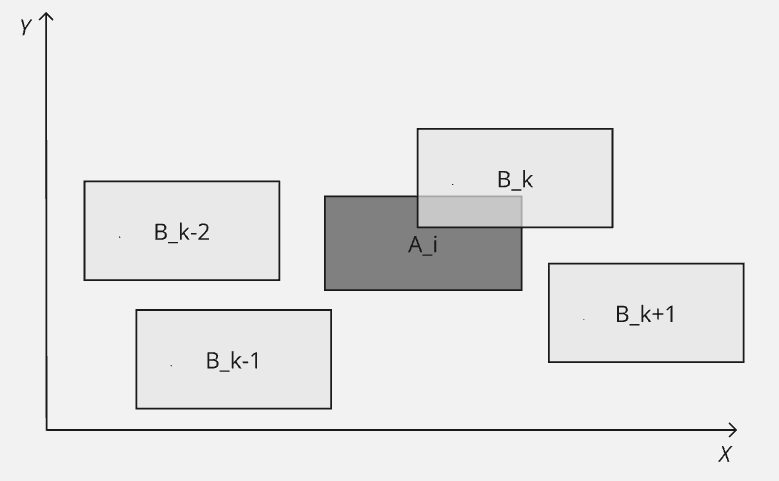
\includegraphics[width=0.75\linewidth]{figures/Optimazaciones/Interseccion/interseccion1a1.png}\par
    \caption{Ejemplificación de una iteración del proceso de intersección sobre dos conjuntos A y B.}
    \label{fig:int-graf}
\end{figure}

En algún punto, puede que se alcance un valor $k$, con $0 \leq k < \kappa(B)$, tal que el elemento mínimo de $B_k$ sea estrictamente mayor, en su primera dimensión (dimensión $0$), que el elemento máximo de $A_i$, tal como se muestra en la Figura~\ref{fig:criterio-parada}. Por ejemplo, si el mínimo de $B_k$ es $(3,5)$ y el máximo de $A_i$ es  $(2,3)$. En este caso, se pueden derivar las siguientes conclusiones:

\begin{itemize}
     \item La intersección entre $A_i$ y $B_k$ resulta vacía, ya que todos los valores de $A_i$ tienen un valor menor o igual que el máximo de $A_i$ en la primera dimensión y todos los valores de $B_k$ tienen un valor mayor o igual que el mínimo de $B_k$ en la primera dimensión.
    
    \item Debido al orden creciente de los conjuntos por el operador $<$ de multi-intervalos, cualquier multi-intervalo $B_{k'}$ con $k < k' < \kappa(B)$ tendrá en la primera dimensión de su mínimo un valor mayor o igual que el mínimo de $B_k$ en dicha dimensión, lo cual garantiza que también será vacía su intersección con $A_i$.
\end{itemize}

\begin{figure}[h]
    \centering
    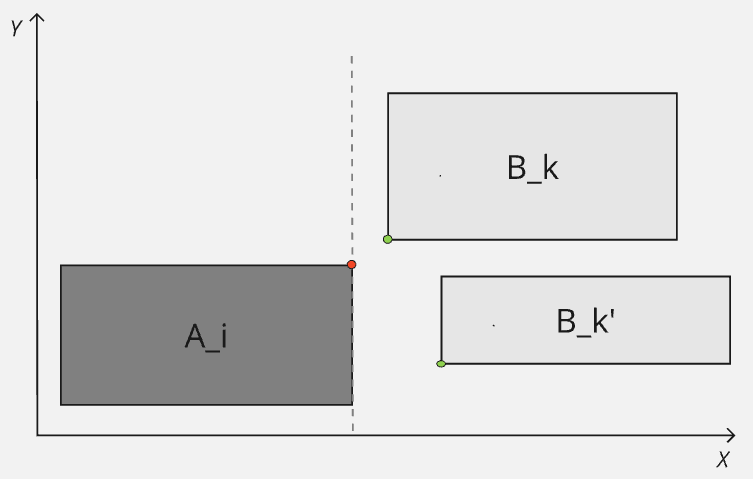
\includegraphics[width=0.75\linewidth]{figures/Optimazaciones/Interseccion/criterio de parada.png}
    \caption{Criterio de parada.}
    \label{fig:criterio-parada}
\end{figure}

En consecuencia, se puede establecer el siguiente criterio fundamental para optimizar la intersección entre conjuntos ordenados:

\begin{center}
    \fbox{
        \parbox{0.92\linewidth}{
            \centering
            \textbf{Criterio de parada} \\[1ex]
            \raggedright
            Sean $A$ y $B$ dos conjuntos ordenados. Supóngase que se está evaluando la intersección entre ambos, y en particular se consideran las posibles intersecciones entre un multi-intervalo $A_i$ de $A$, con $0 \leq i < \kappa(A)$, y los multi-intervalos de $B$. Dado un índice $k$ tal que $0 \leq k < \kappa(B)$, vale lo siguiente:

            \vspace{0,5cm}
     
            \textbf{Si} el máximo de $A_i$ es estrictamente menor que el mínimo de $B_k$ en la primera dimensión, \textbf{entonces}:

            \begin{itemize}
                \item la intersección entre $A_i$ y $B_{k'}$ resulta vacía, $\forall k' \mid k \leq k' < \kappa(B)$,
                \item \textbf{y, entonces} puede continuarse directamente con la evaluación de las intersecciones entre $A_{i+1}$(si existe) y los elementos de $B$.
            \end{itemize}
    
        }
    }
\end{center}

{\bf Criterio de eliminación}

\begin{center}
    \textit{Nuevamente, supóngase que se lleva a cabo la intersección entre $A$ y $B$, dos conjuntos ordenados, y se están considerando las posibles intersecciones del multi-intervalo \( i \)-ésimo de $A$, \( A_i \), con todos los multi-intervalos de $B$.}
\end{center}

En algún punto, puede que se alcance un valor $k$, con $0 \leq k < \kappa(B)$, tal que el elemento máximo de $B_k$ sea estrictamente menor, en su primera dimensión (dimensión $0$), que el elemento mínimo de $A_i$, tal como se muestra en la Figura~\ref{fig:criterio-eliminacion}. Por ejemplo, si el mínimo de $A_i$ es $(3,5)$ y el máximo de $B_k$ es  $(2,3)$. En este caso, se pueden derivar las siguientes conclusiones:

\begin{itemize}
     \item La intersección entre $A_i$ y $B_k$ resulta vacía, ya que todos los valores de $A_i$ tienen un valor mayor o igual que el mínimo de $A_i$ en la primera dimensión y todos los valores de $B_k$ tienen un valor menor o igual que el máximo de $B_k$ en la primera dimensión.

    \item Debido al orden creciente de los conjuntos por el operador $<$ de multi-intervalos, cualquier multi-intervalo $A_{i'}$ con $i < i' < \kappa(A)$ tendrá en la primera dimensión de su mínimo un valor mayor o igual que el mínimo de $A_i$ en dicha dimensión, lo cual garantiza que también será vacía su intersección con $B_k$.
\end{itemize}

\begin{figure}[h]
    \centering
    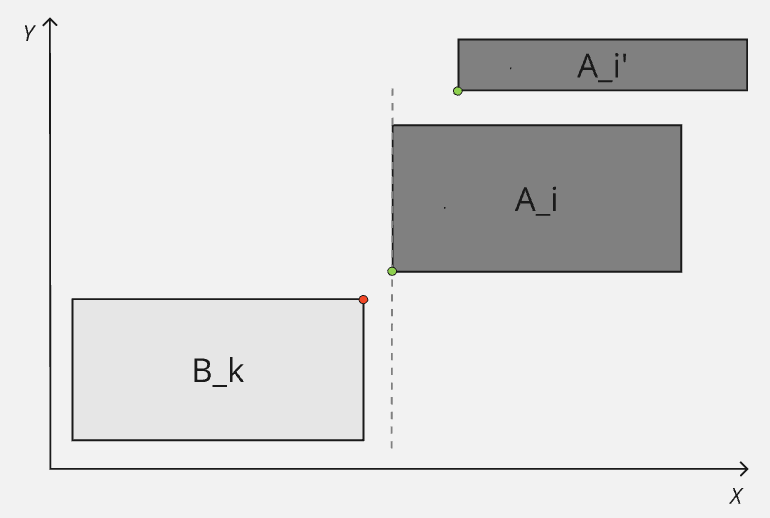
\includegraphics[width=0.75\linewidth]{figures/Optimazaciones/Interseccion/criterio de elim.png}
    \caption{Criterio de eliminación.}
    \label{fig:criterio-eliminacion}
\end{figure}

En consecuencia, se puede establecer el siguiente criterio fundamental para optimizar la intersección entre conjuntos ordenados:


\begin{center}
    \fbox{
        \parbox{0.92\linewidth}{
            \centering
            \textbf{Criterio de eliminación} \\[1ex]
            \raggedright
            Sean $A$ y $B$ dos conjuntos ordenados. Supóngase que se está evaluando la intersección entre ambos, y en particular se consideran las posibles intersecciones entre un multi-intervalo $A_i$ de $A$, con $0 \leq i < \kappa(A)$, y los multi-intervalos de $B$. Dado un índice $k$ tal que $0 \leq k < \kappa(B)$, vale lo siguiente:

            \vspace{0,5cm}
     
            \textbf{Si} el máximo de $B_k$ es estrictamente menor que el mínimo de $A_i$ en la primera dimensión, \textbf{entonces}:

            \begin{itemize}
                \item la intersección entre $A_{i'}$ y $B_{k}$ resulta vacía, $\forall i' \mid i \leq i' < \kappa(A)$,
                
                \item \textbf{y, entonces} puede descartarse $B_k$ para los cálculos de las posibles intersecciones de los multi-intervalos posteriores a $A_i$.
            \end{itemize}
    
        }
    }
\end{center}

Cabe señalar que, tanto para este criterio como para el anterior, no se especifica el tipo de multi-intervalo (si es denso o no), ya que dicha característica no afecta directamente la validez de los mismos.


{\bf Criterio de selección}

Tal como se analizó en el criterio de eliminación, el procedimiento de intersección considera cada multi-intervalo del conjunto $A$ e intenta intersectarlo con todos los multi-intervalos del conjunto $B$. Y donde la idea central del criterio es que, a medida que se avanza en este proceso, ciertos elementos de $B$ pueden ser descartados progresivamente si se determina que ya no podrán intersectar con los siguientes elementos de $A$.

Naturalmente, se puede llegar al punto en el cual todos los elementos de $B$ habrán sido descartados, lo que implica que la operación \texttt{intersection} podrá finalizar directamente ya que no quedan intersecciones posibles a verificar.

Ahora bien, existe una observación importante respecto al tamaño de $B$: cuanto menor sea la cantidad de multi-intervalos en $B$, más rápido podrán descartarse todos ellos posiblemente, y por tanto, terminar la operación.

En base a esta idea, se introduce el \textbf{criterio de selección}, el cual establece lo siguiente:

\begin{center}
    \fbox{
        \parbox{0.9\linewidth}{
            \centering
            \textbf{Criterio de selección} \\[1ex]
            \raggedright
            Sean dos conjuntos ordenados involucrados en la operación de intersección. Se establece lo siguiente:

            \begin{center}
            \textit{
                Se define como $B$ a aquel conjunto que contiene la menor cantidad de multi-intervalos,
                mientras que se denota como $A$ al conjunto restante.
            }
            \end{center}
        }
    }
\end{center}

{\bf Criterio de solapamiento}


Se introduce ahora el \textbf{criterio de solapamiento}, el cual establece lo siguiente:

\begin{center}
    \fbox{
        \parbox{0.93\linewidth}{
            \centering
            \textbf{Criterio de solapamiento} \\[1ex]
            \raggedright
            Sean $A$ y $B$ dos conjuntos, $A_i$ un multi-intervalo del conjunto $A$ y $B_k$ un multi-intervalo del conjunto $B$, con índices tales que:
            \[
            0 \leq i < \kappa(A), \quad 0 \leq k < \kappa(B).
            \]
            Se establece entonces que, en el caso de realizar la intersección entre $A$ y $B$:

            \begin{itemize}
                \item \textbf{Si} existe solapamiento entre $A_i$ y $B_k$, \textbf{entonces}:
                \begin{itemize}
                    \item \textbf{Si} ambos multi-intervalos son \textit{densos}, la intersección entre ellos es necesariamente no vacía y debe proceder.
                    \item \textbf{Si} al menos uno de ellos no es denso, la intersección \textit{puede} ser no vacía, pero no se garantiza de modo que se debe proceder de igual manera.
                \end{itemize}

                \item \textbf{Si} \textbf{no} existe solapamiento entre $A_i$ y $B_k$, \textbf{entonces} la intersección entre ellos es necesariamente vacía, independientemente de si son densos o no, y por ende puede obviarse su cálculo.
            \end{itemize}
        }
    }
\end{center}

Ahora bien, seguiría explicar que es el solapamiento en si:

\begin{center}
    \textit{Sean dos multi-intervalos $mdi_1$ y $mdi_2$. Los multi-intervalos $mdi_1$ y $mdi_2$ se \textbf{solapan} \textbf{si}, \textbf{y sólo si}, todos sus intervalos componentes en cada dimensión se solapan.}

    \textit{Sean $a = [a_{\text{begin}} : a_{\text{step}} : a_{\text{end}}]$ y $b = [b_{\text{begin}} : b_{\text{step}} : b_{\text{end}}]$ dos intervalos. Se dice que se \textbf{solapan} \textbf{si}, \textbf{y sólo si}, se cumple la siguiente condición:}

$\neg (b_{\text{end}} < a_{\text{begin}} \lor a_{\text{end}} < b_{\text{begin}})$

\textit{o bien las siguientes dos condiciones:}

$\bullet \;b_{\text{end}} \geq a_{\text{begin}}$ y $\bullet \;a_{\text{end}} \geq b_{\text{begin}}$

\end{center}

Para ejemplificar mejor la noción de solapamiento en intervalos se proponen los siguientes casos en base al predicado presentado por la definición:

\begin{itemize}
    \item \textbf{Caso $b_{\text{end}} < a_{\text{begin}}$ y $a_{\text{end}} \geq b_{\text{begin}}$:}

    En este caso, no hay solapamiento. Por ejemplo, si $b = [1:1:5]$ y $a = [6:2:10]$, entonces $5 < 6$, por lo tanto, no se solapan. Dicho ejemplo se puede ver en la Figura~\ref{fig:ej1}.

    \begin{figure}[h]
        \centering
        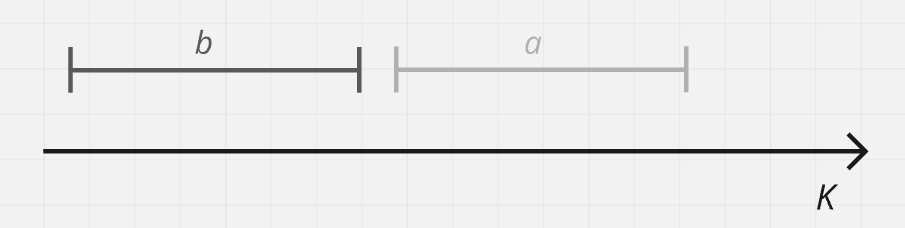
\includegraphics[width=0.75\linewidth]{figures/Optimazaciones/Interseccion/crit sol 10.png}
        \caption{Solapamiento sobre intervalos: \textit{segunda condición verdadera}.}
        \label{fig:ej1}
    \end{figure}

    \item \textbf{Caso $b_{\text{end}} \geq a_{\text{begin}}$ y $a_{\text{end}} < b_{\text{begin}}$:}

    Nuevamente, no hay solapamiento. Por ejemplo, si $b = [8:2:10]$ y $a = [4:2:6]$, entonces $6 < 8$. Este caso se puede observar en la Figura~\ref{fig:ej2}.

    \begin{figure}[h]
        \centering
        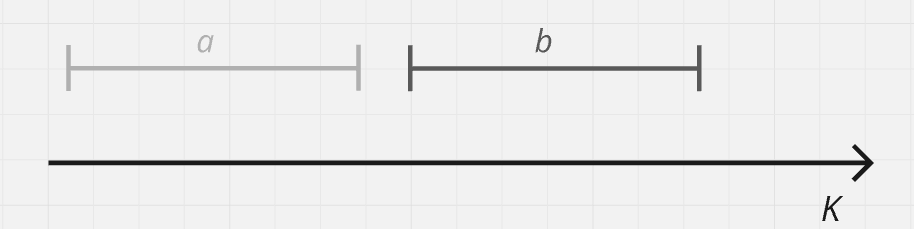
\includegraphics[width=0.75\linewidth]{figures/Optimazaciones/Interseccion/crit sol01.png}
        \caption{Solapamiento sobre intervalos: \textit{primera condición verdadera}.}
        \label{fig:ej2}
    \end{figure}

    \item \textbf{Caso ambas condiciones se cumplen:}

    En este caso resulta que se pueden dar dos situaciones unicamente: $b_{begin}$ o $b_{end}$ se encuentran entre $a_{begin}$ y $a_{end}$ inclusive (Figura~\ref{fig:crit-solapamiento-b}, Figura~\ref{fig:crit-solapamiento-c} y Figura~\ref{fig:crit-solapamiento-d}), ó $b_{begin} < a_{begin}$ y $b_{end}>a_{end}$ (Figura~\ref{fig:crit-solapamiento-a}).

\begin{figure}[H]
    \centering

    \begin{subfigure}{0.75\linewidth}
        \centering
        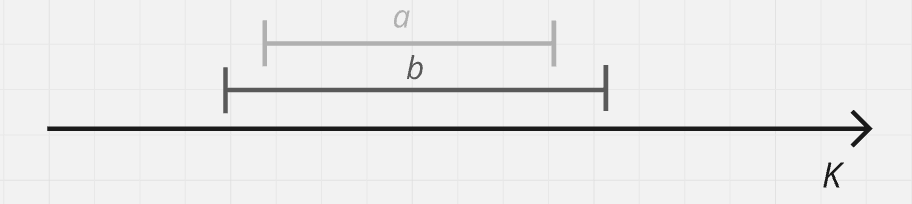
\includegraphics[width=\linewidth]{figures/Optimazaciones/Interseccion/crit sol 11 1.png}
        \caption{}
        \label{fig:crit-solapamiento-a}
    \end{subfigure}
    
    \vspace{0.4cm}

    \begin{subfigure}{0.75\linewidth}
        \centering
        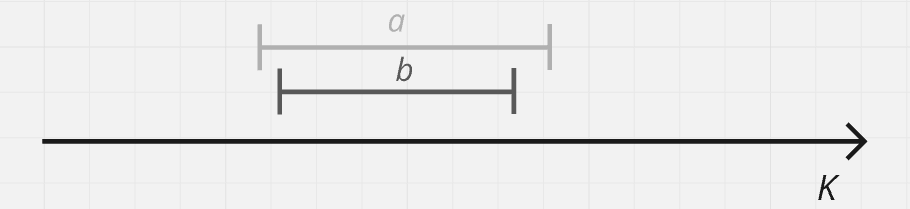
\includegraphics[width=\linewidth]{figures/Optimazaciones/Interseccion/crit sol 11 2.png}
        \caption{}
        \label{fig:crit-solapamiento-b}
    \end{subfigure}
    
    \vspace{0.4cm}

    \begin{subfigure}{0.75\linewidth}
        \centering
        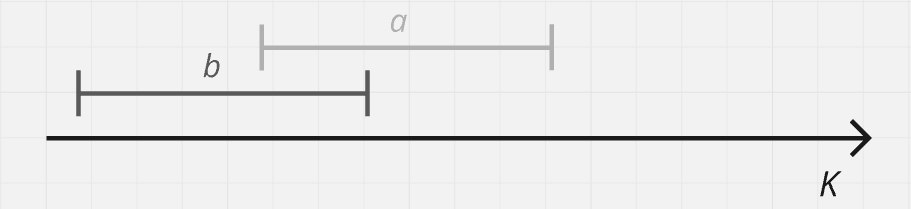
\includegraphics[width=\linewidth]{figures/Optimazaciones/Interseccion/crit sol 11 3.png}
        \caption{}
        \label{fig:crit-solapamiento-c}
    \end{subfigure}
    
    \vspace{0.4cm}

    \begin{subfigure}{0.75\linewidth}
        \centering
        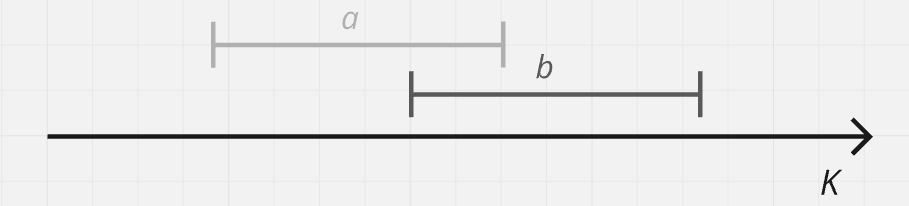
\includegraphics[width=\linewidth]{figures/Optimazaciones/Interseccion/crit sol 11 4.png}
        \caption{}
        \label{fig:crit-solapamiento-d}
    \end{subfigure}

    \caption{Solapamiento sobre intervalos: \textit{ambas condiciones se cumplen}.}
    \label{fig:crit-solapamiento}
\end{figure}
        \item \textbf{Caso ambas condiciones son falsas:}
        
        Cabe destacar que el caso en el cual \textbf{ambas condiciones} sean falsas simultáneamente es imposible. En efecto, si se cumple que:

        \[
        b_{\text{end}} < a_{\text{begin}} \quad \text{y} \quad a_{\text{end}} < b_{\text{begin}},
        \]
        
        entonces, por $a_{\text{begin}} < a_{\text{end}}$ y transitividad de la desigualdad, se deduce que:
        
        \[
        b_{\text{end}} < b_{\text{begin}},
        \]
        
        lo cual implicaría que el intervalo $b$ está mal definido, ya que su extremo final es menor que su extremo inicial. Esto contradice la definición válida de intervalo, por lo tanto, dicho caso \textbf{no} puede ocurrir.
\end{itemize}


Por un lado, se puede observar que si, en al menos una dimensión, los intervalos correspondientes de dos multi-intervalos $mdi$ y $mdi'$, ya sean densos o no, no se solapan, entonces no existe ninguna $n$-upla $(mdi[0], \dots, mdi[n-1]) \in mdi$ y $(mdi'[0], \dots, mdi'[n-1]) \in mdi'$ tal que coincidan en esa dimensión, con $n$ siendo la aridad de $mdi$ y $mdi'$. En consecuencia, esto implica que la intersección entre $mdi$ y $mdi'$ será vacía, independientemente de que en las demás dimensiones sí exista solapamiento.

Por otro lado, si en todas las dimensiones los intervalos correspondientes se solapan y ambos multi-intervalos son densos, entonces se garantiza la existencia de al menos una $n$-upla $(mdi[0], \dots, mdi[n-1])$ perteneciente tanto a $mdi$ como a $mdi'$.

Sin embargo, si uno o ambos multi-intervalos no son densos, esta garantía desaparece. Aunque exista solapamiento en todas las dimensiones, podría no haber ninguna $n$-upla común, ya que en alguna dimensión podría ocurrir que, debido al paso distinto de 1, el intervalo solapamiento puede no tener valores comunes. Por ejemplo, en una dimensión se pueden contar con los intervalos $[5:5:10]$ y $[6:1:9]$, los cuales se solapan, pero cuya intersección es vacía. 

\subsubsection{Criterio de ordenamiento}

Uno de los aspectos fundamentales a considerar al implementar la operación de intersección entre conjuntos ordenados, es cómo construir el conjunto resultado de manera que preserve el orden. En este contexto, el desafío consiste en insertar las intersecciones de los multi-intervalos en el conjunto resultado de la forma más eficiente posible, garantizando siempre que se mantenga la invariante del orden.

\begin{center}
    \fbox{
        \parbox{0.93\linewidth}{
            \centering
            \textbf{Criterio de ordenamiento} \\[1ex]
            \raggedright
            Supóngase que se realiza la intersección entre dos conjuntos ordenados, $A$ y $B$, y que se están evaluando las posibles intersecciones del $i$-ésimo multi-intervalo de $A$, denotado por $A_i$, con todos los multi-intervalos de $B$. Ademas se cuenta con un conjunto resultado $C$.

            \vspace{1ex}

            Todas las intersecciones no vacías generadas con $A_i$ deben insertarse en $C$ \textbf{después} de aquellas intersecciones generadas por los multi-intervalos $A_0, A_1, \dots, A_{i-1}$, cuyos mínimos sean estrictamente menores al de $A_i$, bajo el operador $<$ de naturales multi-dimensionales.
        }
    }
\end{center}


Este criterio se fundamenta en la observación de que la intersección entre dos multi-intervalos está contenida en ambos. Esto implica que el elemento mínimo de la intersección debe ser, necesariamente, un valor que pertenezca a ambos operandos, y por lo tanto debe coincidir con el mínimo de alguno de ellos, o bien ser un valor contenido en ambos.

Al fijar el multi-intervalo $A_i$ como decreta el criterio, se observa que cualquier intersección no vacía con un multi-intervalo $B_k$ del conjunto $B$ tendrá su mínimo dentro de $A_i$, o coincidirá con el mínimo de este. Como resultado, cualquier intersección no vacía generada tendrá un mínimo mayor, bajo el operador $<$ de naturales multi-dimensionales, o igual que el mínimo de $A_i$.

Esto garantiza que tales intersecciones deben insertarse en el conjunto resultado después de aquellas cuyo mínimo sea estrictamente menor, bajo el operador $<$ de naturales multi-dimensionales, al de $A_i$. 

La Figura~\ref{fig:enter-label} ilustra gráficamente esta situación. Como se observa, todas las intersecciones producidas a partir de $A_i$ tienen un mínimo mayor o igual que el de $A_i$, y se insertan a continuación de las intersecciones previamente procesadas cuyo mínimo sea menor al de $A_i$.

\begin{figure}[h]
    \centering
    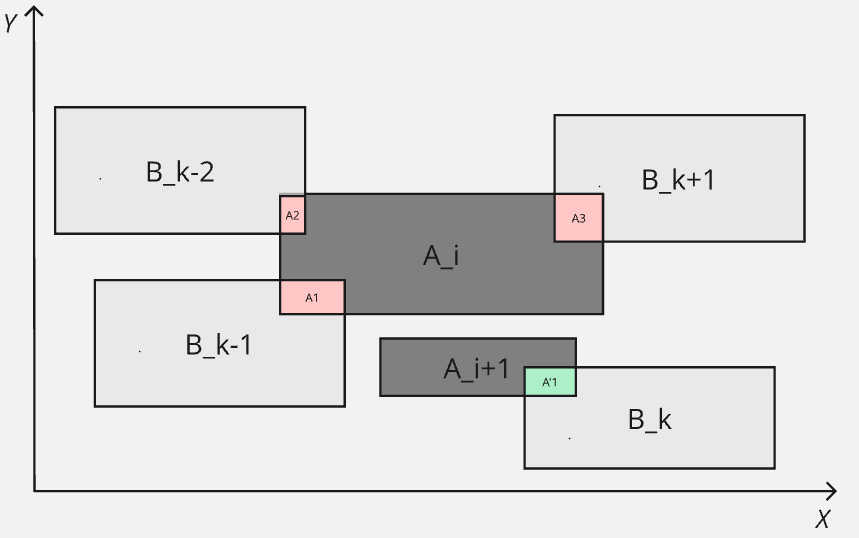
\includegraphics[width=0.7\linewidth]{figures/Optimazaciones/Interseccion/crit ordenamiento.png}
    \caption{Criterio de ordenamiento en la intersección de conjuntos ordenados.}
    \label{fig:enter-label}
\end{figure}

Adicionalmente, no es necesario comenzar a verificar la posición de inserción de las intersecciones en el conjunto resultado desde el principio en cada iteración de los elementos de $A$. Dado el orden intrínseco de los conjuntos involucrados, se cumple que:
\begin{center}
    \textit{El mínimo de $A_i$ es menor, bajo el operador $<$ de naturales multi-dimensionales, al mínimo de $A_{i+1}$}
\end{center}

Esto implica, en conjunto con lo establecido previamente sobre los mínimos de las intersecciones generadas, que todas las intersecciones obtenidas a partir de $A_{i+1}$ con los elementos de $B$ deben insertarse en el conjunto resultado a partir de una posición \textbf{igual o posterior} a aquella en la que comenzaron a insertarse las intersecciones de $A_i$ con $B$.

Por lo tanto, el criterio de ordenamiento puede refinarse del siguiente modo:



\begin{center}
    \fbox{
        \parbox{0.93\linewidth}{
            \centering
            \textbf{Criterio de ordenamiento} \\[1ex]
            \raggedright
            Supóngase que se realiza la intersección entre dos conjuntos ordenados, $A$ y $B$, y que se están evaluando las posibles intersecciones del $i$-ésimo multi-intervalo de $A$, denotado por $A_i$, con todos los multi-intervalos de $B$. Ademas se cuenta con un conjunto resultado $C$.

            \vspace{1ex}

            Todas las intersecciones no vacías generadas con $A_i$ deben insertarse en $C$ \textbf{después} de aquellas intersecciones generadas por los multi-intervalos $A_0, A_1, \dots, A_{i-1}$, cuyos mínimos sean estrictamente menores al de $A_i$, bajo el operador $<$ de naturales multi-dimensionales.
            
            \vspace{1ex}

            Adicionalmente \textbf{si} la posición a partir de la cual se colocan las intersecciones de $A_i$ en el conjunto resultante es $k$, con $0 \leq k < \kappa(C)$, \textbf{entonces} aquellas generadas por $A_{i+1}$ se insertaran a partir de $k'$ tal que $k \leq k' < \kappa(C)$.
        }
    }
\end{center}



Esta optimización reduce significativamente la cantidad de comparaciones necesarias para ubicar cada intersección, manteniendo la eficiencia del proceso y evitando retrocesos innecesarios dentro de la estructura del conjunto ordenado resultante.


\subsection{Unión disjunta - \texttt{disjointCup}}

La operación \texttt{disjointCup} se encarga de realizar la unión disjunta entre dos conjuntos de multi-intervalos que, por hipótesis, son disjuntos. En particular, esta operación simplemente coloca los elementos de ambos conjuntos en uno solo, sin aplicar ningún tipo de transformación adicional, ni sobre los argumentos, ni sobre el contenido de sus elementos. Esto se puede ver muy bien particularmente en el pseudocódigo del Algoritmo \ref{alg:disjointcupDes} de esta para conjuntos desordenados.

Ahora bien, al trabajar con conjuntos ordenados, resulta necesario introducir un criterio de ordenamiento que garantice que el conjunto resultante mantenga el orden. Este criterio de ordenamiento se presenta a continuación.

\subsubsection{Criterio de ordenamiento}

\begin{center}
    \fbox{
        \parbox{0.93\linewidth}{
            \centering
            \textbf{Criterio de ordenamiento}\\[1ex]
            \raggedright
            Sean $A = \{A_0, A_1, \dots, A_{n-1}\}$ y $B = \{B_0, B_1, \dots, B_{m-1}\}$ dos conjuntos no vacíos de multi-intervalos, disjuntos y ordenados. Sea $C$ un conjunto ordenado que contendrá el resultado de la fusión de $A$ y $B$. Y sean $A_i$ un multi-intervalo del conjunto $A$ y $B_k$ un multi-intervalo del conjunto $B$, con índices tales que:
            \[
            0 \leq i < \kappa(A), \quad 0 \leq k < \kappa(B).
            \]
            
            \vspace{1ex}

            Entonces, al realizar la unión disjunta entre $A$ y $B$ vale que:

            \begin{itemize}
                \item \textbf{Si $A_i < B_k$}, entonces $A_i$ debe insertarse en $C$ \textbf{antes} que $B_{k'}$ y $A_{i'}$, $\forall i',k' \mid i < i' < \kappa(A) \land k \leq k' < \kappa(B)$.
                \item \textbf{Si $B_k < A_i$}, entonces $B_k$ debe insertarse en $C$ \textbf{antes} que que $B_{k'}$ y $A_{i'}$, $\forall i',k' \mid i \leq i' < \kappa(A) \land k < k' < \kappa(B)$.
            \end{itemize}

            \vspace{1ex}
        }
    }
\end{center}

Este criterio se fundamente por el orden que disponen los conjuntos ordenados y a su vez por la propiedad transitiva que verifica el operador $<$ de multi-intervalos.

\subsection{Complemento - \texttt{complement / complementAtom}}

Esta sub-sección se dividirá en dos partes, ya que la operación de complemento para conjuntos ordenados, al igual que su contraparte de conjuntos desordenados, se compone de dos etapas: el \textit{complemento atómico} (\texttt{complementAtom}), que calcula el complemento de un conjunto ordenado representado por un único multi-intervalo; y el \textit{complemento general} (\texttt{complement}), la operación principal del complemento, que extiende esta operación tal que sea posible calcular el complemento de conjuntos ordenados compuestos por múltiples multi-intervalos sacando provecho de la operación \texttt{intersection}.

\subsubsection{Complemento atómico(\texttt{complementAtom})}

Dentro de la Sub-sección~\ref{sec:conjs-des} se presentó el funcionamiento y la lógica de la construcción del conjunto complemento de un conjunto atómico, un conjunto compuesto por un único multi-intervalo, mediante la operación \texttt{complementAtom}, en el contexto de los conjuntos desordenados.

Tal como se mencionó, la estructura general de la implementación de las operaciones para conjuntos ordenados se basa en la utilizada para conjuntos desordenados. Por esta razón, correspondería ahora optimizar dicha operación teniendo en cuenta el orden y adaptarla para conjuntos ordenados.

Sin embargo, dado que el conjunto base contiene únicamente un multi-intervalo y solo se cuenta con un único conjunto como argumento de la operación, no hay margen para aplicar ninguna optimización basada en el orden de los argumentos de entrada. 

Por lo tanto, la única tarea pendiente es mantener el orden en el resultado, lo cual implica determinar el \textbf{criterio de ordenamiento}.

{\bf Criterio de ordenamiento}

En \texttt{complementAtom} se trabaja con dos tipos de multi-intervalos: \textit{all} y \textit{during}. Las transformaciones sucesivas de estos intervalos conforman el complemento del conjunto atómico. El uso de cada uno es el siguiente:

Sea $i$ un número natural que hace referencia una dimensión entre $0$ y la cantidad de dimensiones del conjunto atómico procesado.
\begin{itemize}
  \item \textbf{\textit{all}}:  
    Construye el multi-intervalo ($\textit{all}_{i,b}$) que va desde $0$ hasta el inicio del multi-intervalo del conjunto en la dimensión $i$, siempre que exista.

  \item \textbf{\textit{during}}:  
    Cuando el multi-intervalo del conjunto no es denso en la dimensión $i$, es decir, el paso de la $i$-esima dimensión ($\text{paso}_i$) es distinto de $1$, se generan una serie de multi-intervalos intermedios ($\textit{during}_{i,c}$). Cada uno arranca en
    \[
      \bigl(\text{begin}_i\bigr) + c,
      \quad c = 1, 2, \dots, (\text{paso}_i - 1),
    \]
    donde $\text{begin}_i$ es el inicio en la dimensión $i$ del multi-intervalo del conjunto.

  \item \textbf{\textit{all}}:  
    Construye el multi-intervalo ($\textit{all}_{i,e}$) que va desde el final del multi-intervalo del conjunto en la dimensión $i$ hasta \texttt{Inf}, siempre que sea posible.
\end{itemize}

Sin embargo, al realizar el procesamiento secuencial de cada dimensión, es necesario tener en cuenta cómo los inicios de los intervalos correspondientes a las dimensiones ya recorridas del multi-intervalo  se propagan hacia $all$ y $during$. 

Una vez completados los cálculos en la dimensión $i$ (creación de \textit{all}$_{i,b}$, \textit{all}$_{i,e}$ y todos los \textit{during}$_{i,c}$), tanto \textit{during} como \textit{all} se modifican en dicha dimensión. A \textit{all} se le remplaza el intervalo en esa dimensión por el del multi-intervalo del conjunto en la misma dimensión pero con paso 1, y a \textit{during} se le hace lo mismo pero con el intervalo original.

Como consecuencia, todos los multi-intervalos que se generen en la siguiente dimensión $i+1$ tienen el mismo valor de inicio en la dimensión $i$ que tiene el multi-intervalo del conjunto. Por lo tanto los inicios de \textit{all}$_{i,b}$, \textit{all}$_{i,e}$ y de cada \textit{during}$_{i,c}$ coinciden, en las dimensiones $0,1,\ldots,i-1$, con los del multi-intervalo atómico original. Lo que conlleva a que el siguiente conjunto este ordenado:

\[
\{\textit{all}_{i,b},\;\textit{during}_{i,1},\;\textit{during}_{i,2},\;\dots,\;\textit{during}_{i,k},\;\textit{all}_{i,e}\}
\]

Pero ahora queda ver que interacción hay entre los conjuntos de cada dimensión para ver como ordenar la totalidad de los multi-intervalos de todas las dimensiones en un único conjunto.

Al estar en una dimensión $i$ y al haber terminado de generar los multi-intervalos de esa dimensión a través de \textit{during} y \textit{all}, por como son las modificaciones a estos dos multi-intervalos, resulta que todos los multi-intervalos generados en la dimensión $i+1$ van inmediatamente después de $all_{i,b}$(si existe), ya que en la dimensión $i$ tiene un valor de inicio $0$. Ademas, se los debe incluir antes de los \textit{during}$_{i,c}$, cuyo inicio en la dimensión $i$ es el mismo que el de los multi-intervalos generados en $i+1$, adicionando una constante $c$. Como resultado tenemos que se da el siguiente orden:

\begin{align*}
\{ &\textit{all}_{x,b},\ \textit{all}_{y,b},\ \textit{all}_{z,b}, \\
   &\textit{during}_{z,1},\ \textit{during}_{z,2},\ \dots,\ \textit{during}_{z,k}, \\
   &\textit{all}_{z,e},\ \textit{during}_{y,1},\ \textit{during}_{y,2},\ \dots,\ \textit{during}_{y,j}, \\
   &\textit{all}_{y,e},\ \textit{during}_{x,1},\ \textit{during}_{x,2},\ \dots,\ \textit{during}_{x,j}, \\
   &\textit{all}_{x,e} \}
\end{align*}

trabajando con un conjunto atómico de tres dimensiones.

A partir de todo lo analizado previamente, se arriba a la siguiente formulación del criterio de ordenamiento para \texttt{complementAtom}:

\begin{center}
    \fbox{
        \parbox{0.93\linewidth}{
            \centering
            \textbf{Criterio de ordenamiento}\\[1ex]
            \raggedright
            El patrón general de inserción en las estructuras auxiliares $all$ y $during$, al recorrer las dimensiones en orden creciente, responde a la siguiente disposición:

            \begin{align*}
            \{ &\textit{all}_{0,b},\ \textit{all}_{1,b},\ \dots,\ \textit{all}_{k-1,b}, \\
               &\textit{during}_{k-1,1},\ \dots,\ \textit{during}_{k-1,u_{i-1}}, \\
               &\textit{all}_{k-1,e},\ \textit{during}_{k-2,1},\ \dots,\ \textit{during}_{k-2,u_{i-2}}, \\
               &\quad\vdots \\
               &\textit{all}_{1,e},\ \textit{during}_{0,1},\ \dots,\ \textit{during}_{0,u_0}, \\
               &\textit{all}_{0,e} \}
            \end{align*}

            \vspace{1ex}

            donde $k$ representa la aridad del conjunto (es decir, la cantidad de dimensiones), y $u_i$ indica la cantidad de pasos definidos en la dimensión $i$.
        }
    }
\end{center}



\subsubsection{Complemento general}

La operación \texttt{intersection} se utiliza como herramienta para calcular el complemento entre dos conjuntos desordenados en la operación \texttt{complement}: uno que representa el complemento de un conjunto de multi-intervalos desordenados, y otro que representa el complemento de un conjunto con un único multi-intervalo.

Teóricamente, podría utilizarse una única implementación general de \texttt{intersection}, como se hace en el caso de conjuntos desordenados y no modificar \texttt{complement} para el caso de conjuntos ordenados. Sin embargo, al tratarse de conjuntos ordenados, es posible aplicar ciertas optimizaciones adicionales, además de algunas de las ya detalladas en la sub-sección correspondiente a \texttt{intersection}, que permiten mejorar el rendimiento de la operación. Es decir, se utilizará una versión adaptada de la intersección de conjuntos ordenados para el complemento.

{\bf Intersección complementaria}

En esta modificación de la operación de intersección, denominada \texttt{intersectionComp}, se preservan los criterios de \textbf{solapamiento} y \textbf{ordenamiento}. Además de suponer que los conjuntos recibidos están ordenados, esta variante introduce una hipótesis adicional: los argumentos deben respetar un orden específico. El primer conjunto debe representar el complemento de un conjunto de multi-intervalos (posiblemente varios), mientras que el segundo conjunto corresponde al complemento de un único multi-intervalo. 

En otras palabras:
\begin{itemize}
    \item El primer conjunto, $A$, actúa como un \emph{complemento acumulado}.
    \item El segundo conjunto, denotado $B$, funciona como un \emph{complemento unitario}.
\end{itemize}

\textbf{Importante:} Para facilitar la siguiente explicación, se asume que los multi-intervalos involucrados son siempre densos.

Supongase ahora que el conjunto $A$ representa el complemento de un único multi-intervalo, al igual que $B$. Esta situación se ilustra en la Figura~\ref{fig:tra}.

\begin{figure}[htbp]
    \centering
    \begin{minipage}[t]{0.49\textwidth}
        \centering
        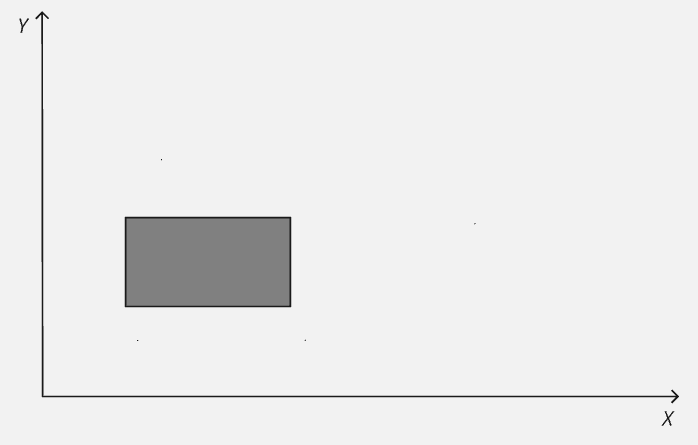
\includegraphics[width=\linewidth]{figures/Optimazaciones/Complement/Aelem.png}
        \caption*{\small Multi-intervalo generador de $A$}
        \vspace{8pt}
        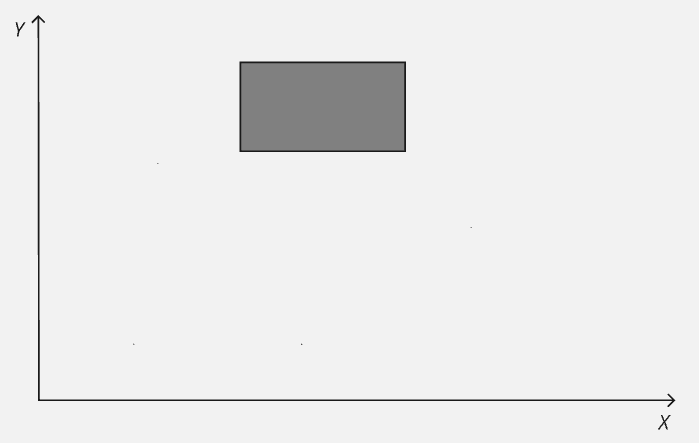
\includegraphics[width=\linewidth]{figures/Optimazaciones/Complement/Belem.png}
        \caption*{\small Multi-intervalo generador de $B$}
    \end{minipage}%
    \hspace{0.01\textwidth}
    \begin{minipage}[t]{0.49\textwidth}
        \centering
        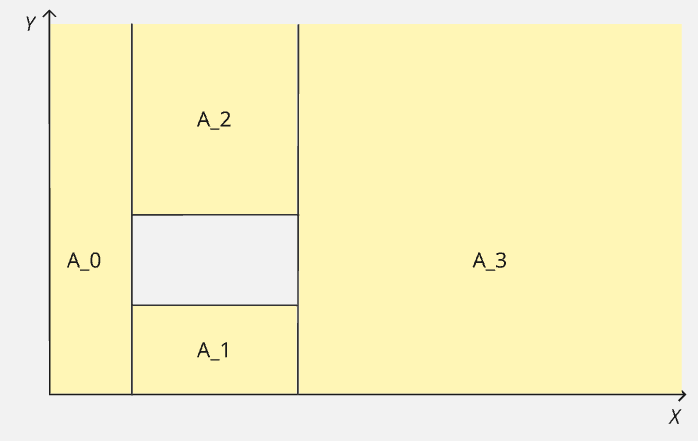
\includegraphics[width=\linewidth]{figures/Optimazaciones/Complement/A.png}
        \caption*{\small Conjunto complemento $A$}
        \vspace{8pt}
        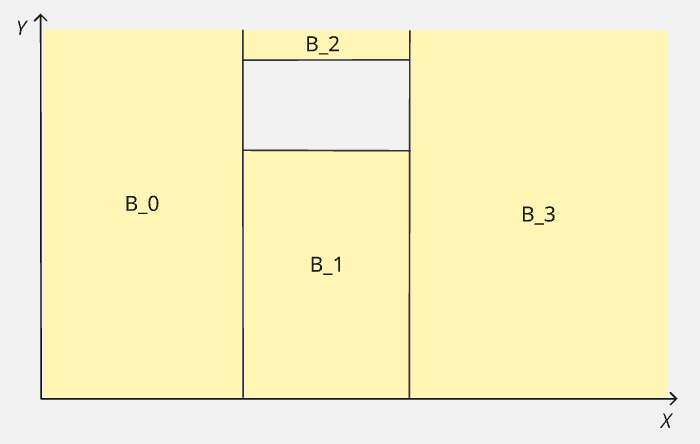
\includegraphics[width=\linewidth]{figures/Optimazaciones/Complement/B.png}
        \caption*{\small Conjunto complemento $B$}
    \end{minipage}
    \caption{Ejemplo gráfico de los conjuntos complemento de $A$ y $B$.}
    \label{fig:tra}
\end{figure}

Si se aplicara directamente la operación \texttt{intersection}, utilizando su versión optimizada para conjuntos ordenados, el resultado obtenido sería el ilustrado en la Figura~\ref{fig:compleAnt}. 

Sin embargo, puede observarse que se produce una partición adicional innecesaria: los multi-intervalos $C\_1$ y $C\_3$ podrían haberse mantenido como un único multi-intervalo. Esta fragmentación/particionamiento es consecuencia del funcionamiento de la operación intersección. No obstante, ambos multi-intervalos no comparten ningún elemento con el multi-intervalo generador de $B$, por lo que no deberían verse afectados ni sufrir ninguna sustracción de elementos al quitar de $A$ los elementos del multi-intervalo generador de $B$ a través de la intersección de $A$ y $B$.


\begin{figure}[htbp]
    \centering
    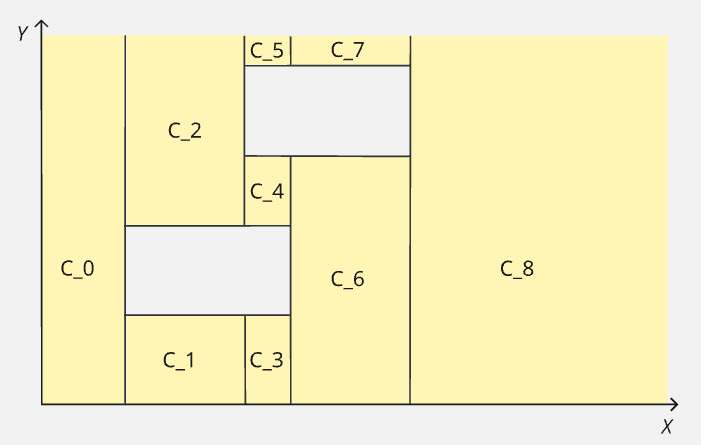
\includegraphics[width=0.8\linewidth]{figures/Optimazaciones/Complement/complAnt.png}
    \caption{Conjunto complemento resultante de la intersección entre $A$ y $B$, sin aplicar optimización.}
    \label{fig:compleAnt}
\end{figure}

Este tipo de fragmentación innecesaria puede evitarse mediante el criterio de optimización denominado \textbf{criterio de anti-particionamiento}, que establece lo siguiente:

\begin{center}
    \fbox{
        \parbox{0.93\linewidth}{
            \centering
            \textbf{Criterio de anti-particionamiento} \\[1ex]
            \raggedright
            Sea $A$ un conjunto complemento y $B$ el complemento de un conjunto compuesto por un único multi-intervalo $mdi$. Al realizar la intersección entre $A$ y $B$ durante el cálculo del complemento de un conjunto, se cumple que:
            
            \vspace{1ex}
            Todo multi-intervalo de $A$ que no se solape con el multi-intervalo $mdi$ generado por $B$ no requiere ser intersectado con los elementos de $B$, y debe copiarse directamente al conjunto resultado.
        }
    }
\end{center}


Aplicando este criterio, el conjunto complemento resultante se muestra en la Figura~\ref{fig:compleNue}, donde se observa una representación más compacta: se evita una partición innecesaria y se obtiene un conjunto más chico.

\begin{figure}[htbp]
    \centering
    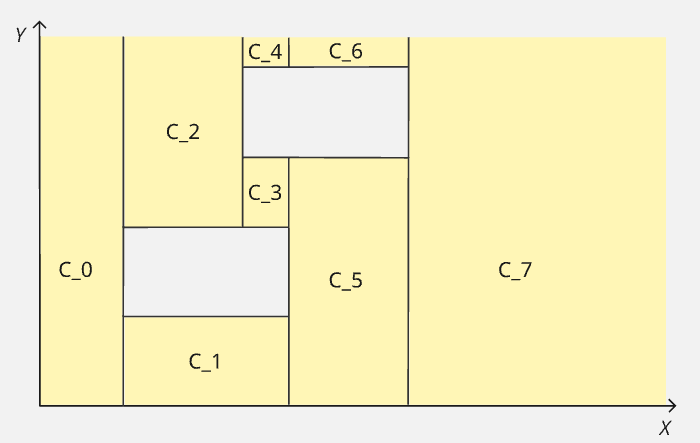
\includegraphics[width=0.8\linewidth]{figures/Optimazaciones/Complement/complNue.png}
    \caption{Conjunto complemento resultante tras aplicar el criterio de anti-particionamiento.}
    \label{fig:compleNue}
\end{figure}

Cabe destacar que este criterio también es válido cuando se trabaja con multi-intervalos no densos, y resulta especialmente útil en esos casos, ya que evita múltiples operaciones de posicionamiento y comparación innecesarias.

Si bien la reducción en el número de multi-intervalos resultantes puede parecer ínfima, es importante tener en cuenta que en la operación \texttt{complement} se aplica de forma acumulativa esta reducción. Por lo tanto, reducir la cantidad de particiones en cada iteración tiene un efecto significativo en el rendimiento total, ya que disminuye la cantidad de elementos a recorrer y comparar en las iteraciones posteriores.

Existe además una mejora adicional que puede aplicarse a la operación de intersección en el contexto del complemento. Esta surge por el modo en que se construye el complemento ordenado de un conjunto atómico, tal como se explicó en la subsección correspondiente del complemento atómico.

En dicha construcción, el primer multi-intervalo del complemento ordenado es $\textit{all}_{x,b}$. Este multi-intervalo es denso y se extiende hasta el infinito en todas sus dimensiones, con excepción de la primera, donde finaliza una posición antes del comienzo del multi-intervalo original que dio lugar al complemento.

Adicionalmente se cumple que la intersección entre cualquier multi-intervalo y uno denso, que lo contiene por completo, es simplemente el multi-intervalo contenido. Es decir, si un multi-intervalo $mdi$ está completamente contenido en otro multi-intervalo denso $mdi'$, entonces la intersección entre $mdi$ y $mdi'$ es igual a $mdi$.

A partir de las observaciones anteriores, puede establecerse el criterio de optimización denominado \textbf{criterio de obviedad}, el cual permite evitar cálculos innecesarios durante la intersección del complemento, y estipula lo siguiente:

\begin{center}
    \fbox{
        \parbox{0.93\linewidth}{
            \centering
            \textbf{Criterio de obviedad} \\[1ex]
            \raggedright
            Sea $A$ un conjunto complemento y $B$ el complemento de un conjunto compuesto por un único multi-intervalo $mdi$. Al realizar la intersección entre $A$ y $B$ durante el cálculo del complemento de un conjunto, se cumple que:

            \vspace{0,5cm}
            
            Todo multi-intervalo del conjunto $A$ cuyo máximo sea estrictamente menor en la primera dimensión que el mínimo multi-intervalo generador de $B$, $mdi$, puede incorporarse directamente al conjunto resultado de la intersección, sin necesidad de ser intersectado con los elementos de $B$.
        }
    }
\end{center}


\begin{comment}
    

\begin{figure}[htbp]
    \centering
    \begin{minipage}[t]{0.49\textwidth}
        \centering
        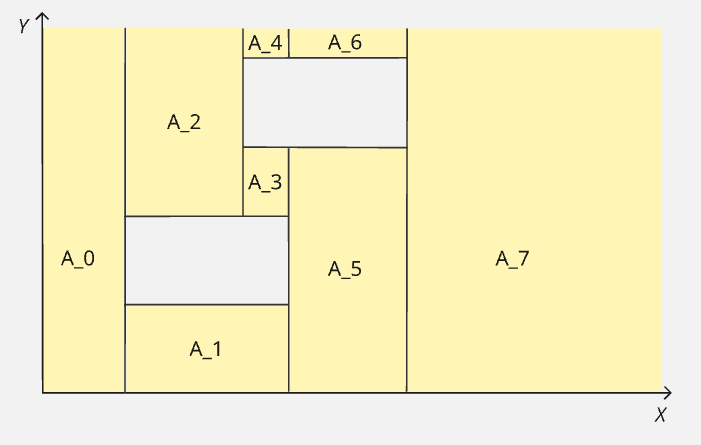
\includegraphics[width=\linewidth]{figures/Optimazaciones/Complement/Ao.png}
        \caption*{\small Conjunto complemento $A$}
    \end{minipage}%
    \hspace{0.01\textwidth}
    \begin{minipage}[t]{0.49\textwidth}
        \centering
        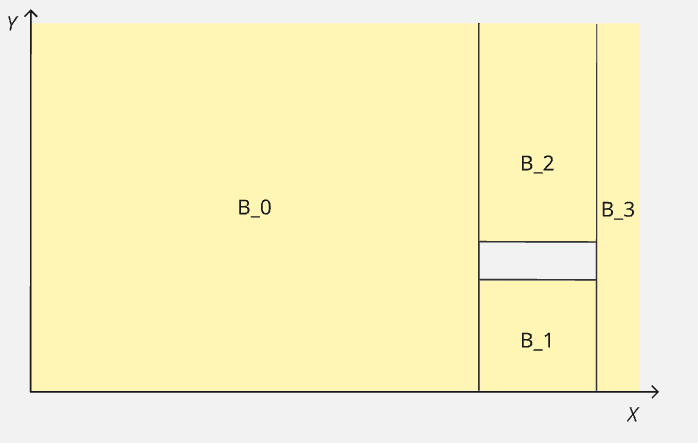
\includegraphics[width=\linewidth]{figures/Optimazaciones/Complement/Bo.png}
        \caption*{\small Conjunto complemento $B$}
    \end{minipage}
    \hspace{0.01\textwidth}
    \begin{minipage}[t]{0.49\textwidth}
        \centering
        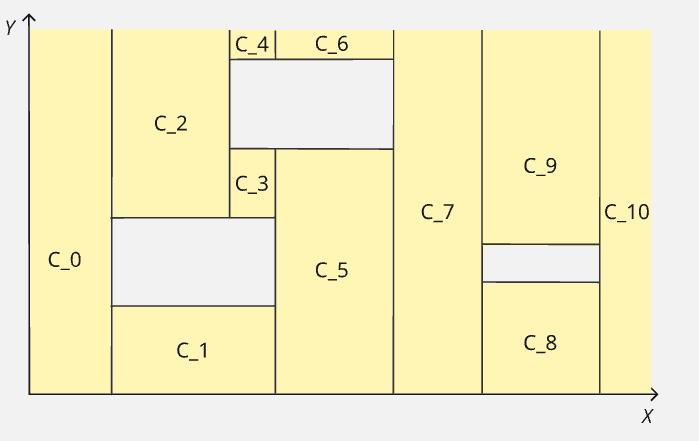
\includegraphics[width=\linewidth]{figures/Optimazaciones/Complement/complO.png}
        \caption*{\small Conjunto complemento resultante de la intersección}
    \end{minipage}
    \caption{Ejemplo gráfico de los conjuntos complemento $A$ y $B$.}
    \label{fig:tra}
\end{figure} 
\end{comment}


Tal como fue planteado, el \textbf{criterio de obviedad} permite evitar las comparaciones e intersecciones entre determinados multi-intervalos del conjunto complemento $A$ y los elementos del conjunto complemento $B$, pero su alcance inicial es limitado: únicamente evita el procesamiento de los multi-intervalos de $A$ que sean estrictamente menores (en la primera dimensión) que el multi-intervalo generador de $B$ en una única invocación de la operación \texttt{intersectionComplement}.

Sin embargo, este criterio puede extenderse de forma significativa durante el proceso iterativo de la operación \texttt{complement}. Esto es posible gracias a la siguiente observación: los multi-intervalos que generan cada conjunto $B$ a lo largo de las distintas iteraciones provienen de un conjunto ordenado, por lo tanto, sus valores iniciales en la primera dimensión son no decrecientes. Dado que estos multi-intervalos se recorren en orden, cada nuevo multi-intervalo generador $B$ tendrá en la primera dimensión un valor de inicio igual o mayor que el anterior. Y, por ende cada nuevo $\textit{all}_{x,b}$ del conjunto $B$ generado por un multi-intervalo contendrá a todos los anteriores $\textit{all}_{x,b}$.

Como consecuencia, una vez que un multi-intervalo de $A$ ha sido descartado por el criterio de obviedad en una iteración, puede descartarse definitivamente para todas las iteraciones subsiguientes, ya que siempre será obviado por el criterio obviedad.

Esto permite trasladar dichos multi-intervalos directamente al resultado final de la operación \texttt{complement}, en lugar de seguirlos incorporando los en el cálculo de las posteriores iteraciones.

Se procede entonces a declarar el \textbf{criterio de obviedad extendido}:

\vspace{10pt}

\begin{center}
    \fbox{
        \parbox{0.93\linewidth}{
            \centering
            \textbf{Criterio de obviedad extendido} \\[1ex]
            \raggedright
            Sea $A$ un conjunto ordenado de multi-intervalos que representa el complemento acumulado en una iteración de la operación \texttt{complement} y $B$ el complemento de un conjunto compuesto por un único multi-intervalo de dicha iteración también.

            \vspace{0,5cm}
            
            Entonces, $A$ puede \textit{descomponerse} en dos subconjuntos disjuntos:
            \begin{itemize}
                \item $A\_o$: el subconjunto de multi-intervalos que son descartados por el criterio de obviedad en base a $B$ en dicha iteración, y que, por lo tanto, pueden ser incorporados directamente al resultado final sin necesidad de ser procesados en iteraciones posteriores;

                
                \item $A\_r$: el subconjunto restante, compuesto por los multi-intervalos que aún pueden ser particionados en iteraciones futuras, es decir, aquellos que no son descartados por el criterio de obviedad en base a $B$. Luego, la intersección se dará entre este conjunto y $B$, y su resultado será el nuevo $A$.
            \end{itemize}
        }
    }
\end{center}

Este criterio permite ahorrar el recorrer los mismos elementos múltiples veces durante el calculo de la intersección e el complemento. Esto permite aumentar en gran medida la eficiencia de la operación.

\section{Implementaciones}

Para llevar a cabo la implementación de los conjuntos ordenados, fue necesario desarrollar una serie de funciones adicionales. A continuación, se describen dichas implementaciones complementarias junto con su correspondiente pseudocódigo.

\subsection{Calculo de solapamiento - \texttt{doInt}}

La operación \texttt{doInt} se utiliza en el contexto de conjuntos ordenados, aunque no forma parte de su interfaz de operaciones. Esta tiene el objetivo de calcular si existe solapamiento entre dos multi-intervalos. Esta operación resulta fundamental tanto para la aplicación del \textbf{criterio de solapamiento} como para el \textbf{criterio de anti-particionamiento}.

El pseudocódigo correspondiente a esta operación se presenta a continuación, y resulta relativamente breve:


\begin{algorithm}
\caption{Cálculo de solapamiento para conjuntos ordenados}
\begin{algorithmic}[1]
\Require $Mdi\_1$ y $Mdi\_2$ son dos multi-intervalos
\Ensure Devuelve \texttt{true} si estos se solapan, \texttt{false} en caso contrario.
\Function{doInt}{$Mdi\_1, Mdi\_2$}

    \
    
    \State $max\_1 :=$ \Call{maxElem}{$Mdi\_1$}
    \State $min\_1 :=$ \Call{minElem}{$Mdi\_1$}
    \State $max\_2 :=$ \Call{maxElem}{$Mdi\_2$}
    \State $min\_2 :=$ \Call{minElem}{$Mdi\_2$}
    \State $a :=$ \Call{arity}{$Mdi\_1$}

    \

    \For{$i = 0$; $i < a-1$ ; $i \!+\!+$}
         \If{$max\_1[i] < min\_2[i]$ \textbf{or} $max\_2[i] < min\_1[i]$}
            \State \Return \texttt{false} 
        \EndIf
    \EndFor

    \
    
    \State \Return \texttt{true} 

\EndFunction
\end{algorithmic}
\end{algorithm}

\subsection{Inserción con pista - \texttt{emplaceHint}}

La función \texttt{emplaceHint} se propone también como una herramienta auxiliar externa a la estructura principal de conjuntos ordenados. Su tarea consiste en insertar un multi-intervalo en un conjunto ordenado, siguiendo el mismo criterio de ordenamiento utilizado por los mismos. Para hacerlo, utiliza una posición pista (\textit{hint}), es un número natural y una posición sugerida y que sirve como punto de inicio para encontrar eficientemente la ubicación correcta del multi-intervalo.

El pseudocódigo de esta función es corto, ya que su implementación es simple, y se encuentra en el Algoritmo \ref{alg:emplaceHint-conj}.

\begin{algorithm}
\caption{Inserción con pista para conjuntos ordenados}
\label{alg:emplaceHint-conj}
\begin{algorithmic}[1]
\Require $A$ es una conjunto ordenado, $Mdi$ en un multi-intervalo y $Hint$ es un numero natural y una posición sugerida.
\Ensure Inserta el $Mdi$ dentro del conjunto ordenado, manteniendo el orden y empezando a buscar la posición de inserción a partir de $Hint$.
\Function{emplaceHint}{$A,Mdi,Hint$}
     \State $n :=$ \Call{size}{$A$}
    \State $it := Hint$ 
    \While{$it < n$}
        \If{$A_{it} < mdi$}
            \State $it$ \!+\!+
        \Else
            \State \textbf{break}
        \EndIf
    \EndWhile

      \State $A :=$ $A_{0:it-1} \frown \{mdi\} \frown A_{it:\Call{size}{A}-1}$
\EndFunction
\end{algorithmic}
\end{algorithm}


\subsection{Avance con pista - \texttt{advanceHint}}

La función \texttt{advanceHint} se propone también como una herramienta auxiliar externa a la estructura principal de conjuntos ordenados. El objetivo de esta función es avanzar la posición de la pista (hint) que viene como argumento en función de los elementos presentes en un conjunto ordenado, utilizando un multi-intervalo como criterio de parada.

El pseudocódigo de esta función auxiliar se presenta a continuación.


\begin{algorithm}
\caption{Avance con pista para conjuntos ordenados}
\label{alg:advanceHint}
\begin{algorithmic}[1]
\Require $A$ es un conjunto ordenado, $Mdi$ en un multi-intervalo y $Hint$ es un número natural.
\Ensure Avanza la pista $Hint$ en base a los elementos del conjunto y el $Mdi$.
\Function{advanceHint}{$A,Mdi,Hint$}
    \State $n :=$ \Call{size}{$A$}
    
    \While{$Hint < n$}
        \If{$A_{Hint} < Mdi$}
            \State $Hint$ \!+\!+
        \Else
            \State \textbf{break}
        \EndIf
    \EndWhile
\EndFunction
\end{algorithmic}
\end{algorithm}



\section{Implementaciones}

Llegado este punto, es momento de abordar las implementaciones concretas de las distintas operaciones sobre conjuntos ordenados. 

Esta seccion se organiza en tres sub-secciones principales: una dedicada a aquellas operaciones cuya implementación no requirió modificaciones, una sub-sección que aborda las operaciones adaptadas para poder funcionar correctamente en el contexto de conjuntos ordenados, y finalmente otra correspondiente a las operaciones que fueron optimizadas.

\subsection{Operaciones sin cambios}

Al implementar los conjuntos ordenados utilizando como base la versión desordenada, se observó que ciertas operaciones no podían beneficiarse del orden para su optimización o no se podían optimizar en si, pero tampoco alteraban dicho orden. Esto se debe, principalmente, a dos razones: o bien son operaciones que no devuelven un conjunto ordenado, o bien el conjunto resultante ya se encuentra ordenado.

Dentro del primer conjunto de operaciones se incluyen, por ejemplo: \texttt{cardinal}, que devuelve el número de elementos que contiene el conjunto; \texttt{arity}, que informa la aridad del mismo; entre otras.

Dado que estas operaciones son numerosas y su comportamiento no resulta central para los objetivos de esta tesina, además de que sus implementaciones se mantuvieron sin modificaciones, no se detallarán aquí. Todas ellas pueden consultarse en el archivo \textit{set.cpp}, disponible en el repositorio dentro de la carpeta \textit{sbg}.

En el segundo conjunto se incluyen operaciones como \texttt{compact}, cuyo algoritmo no elimina el orden del conjunto resultante, o \texttt{cup}, cuya lógica interna se basa exclusivamente en operaciones que preservan dicho orden.

Al igual que en el caso anterior, se omite un desarrollo mas amplio de estas operaciones. Si se desea consultarlas en profundidad puede dirigirse al archivo \textit{set.cpp}, disponible en el repositorio dentro de la carpeta \textit{sbg}.

\subsection{Operaciones adaptadas al orden}

Este grupo de operaciones fueron adaptadas para funcionar en el contexto de conjuntos ordenados, pero no pudieron ser optimizadas. Dentro de estas operaciones se encuentran:

\begin{itemize}
    \item \texttt{emplace}: Que se encarga de ubicar un multi-intervalo dentro de un conjunto.
    \item \texttt{emplaceBack}: Que se encarga de ubicar un multi-intervalo al final de un conjunto, como su último elemento, aquel con mayor mínimo.
    \item \texttt{minElem}: Busca el mínimo mínimo de todos los multi-intervalos de un conjunto
\end{itemize}

Si se desea ver cuales fueron sus modificaciones con respecto a sus versiones de conjuntos desordenados, puede verifica el archivo \textit{set.cpp} dentro de la carpeta \textit{sbg}, disponible en el repositorio.

\subsection{Operaciones optimizadas}

En esta sub-sección se presentan aquellas operaciones que pudieron ser optimizadas aprovechando el orden de los conjuntos. Cada una de ellas será descripta minuciosamente y explicada en detalle, destacando los criterios de optimización y ordenamiento en cada caso.

\subsubsection{Intersección - \texttt{intersection}}
Como se puede observar a continuación, la operación \texttt{intersection} resultó ser considerablemente más extensa que su homóloga para conjuntos desordenados.

No obstante, teniendo en cuenta lo expuesto en la Sub-sección~\ref{sec:opts-int}, se tiene lo siguiente:

\begin{itemize}
    \item Para implementar el \textbf{criterio de selección}, se realiza la verificación correspondiente según lo establecido por dicho criterio: se analiza la cantidad de multi-intervalos presentes en los conjuntos $C$ y $D$. A partir de esta comparación, se determina cuál es el conjunto largo, $A$, y cuál el corto, $B$, tal como se muestra en el Algoritmo \ref{alg:int-ord-1}, líneas 12 a 17.

    \item En relación con el \textbf{criterio de eliminación}, dado que su cumplimiento implica la remoción de un elemento de uno de los conjuntos, en este caso del conjunto $B$, y dado que no es posible eliminar elementos directamente del mismo, se utiliza una lista enlazada que contiene los índices que referencian a los multi-intervalos de $B$. Esto permite llevar a cabo la eliminación de los índices en vez de los multi-intervalos. La preparación de dicha lista se observa en el Algoritmo \ref{alg:int-ord-1}, líneas 18 a 21, y la implementación del criterio se detalla en el Algoritmo \ref{alg:int-ord-2}, líneas 7 a 10.

    \item En cuanto el \textbf{criterio de parada} este se implementa de la linea 11 a 13 en el Algoritmo \ref{alg:int-ord-2}, donde lo único que se hace es forzar la salida del segundo bucle a través de un \texttt{break}.

    \item Para la aplicación del \textbf{criterio de solapamiento}, se emplea la función auxiliar \texttt{doInt}, encargada de verificar si dos multi-intervalos se solapan. Esto se encuentra en el Algoritmo \ref{alg:int-ord-2}, línea 14.

    \item Finalmente, el \textbf{criterio de ordenamiento} se implementa mediante las funciones auxiliares \texttt{advanceHint} y \texttt{emplaceHint}, permitiendo que al aplicar el criterio, el conjunto resultado se mantenga ordenado a lo largo de la ejecución. Esto puede observarse en el Algoritmo \ref{alg:int-ord-2}, líneas 3 y 17.
\end{itemize}

\begin{algorithm}
\caption{Intersección de conjuntos ordenados — Parte 1: Preparación}\label{alg:int-ord-1}
\begin{algorithmic}[1]
\Require $C$ y $D$ son conjuntos ordenados
\Ensure $R$ es la intersección ordenada de $C$ y $D$
\Function{intersection}{$C, D$}
    \State $R := \{\}$

    \If{$\Call{isEmpty}{C}$ \textbf{or} $\Call{isEmpty}{D}$}
        \State \Return{$R$}
    \EndIf

    \If{$C == D$}
        \State \Return{$C$}
    \EndIf
 
    
    \If{ \Call{maxElem}{$C$} $<$ \Call{minElem}{$D$} $ $\textbf{or}$ $ \Call{maxElem}{$C$} $<$ \Call{minElem}{$D$} }
        \State \Return{$R$}
    \EndIf

    
    \State $B := C$
    \State $A := D$

    \If{\Call{size}{$D$} $<$ \Call{size}{$C$}}
        \State $B := D$
        \State $A := C$
    \EndIf

    \State $indices := []$ \Comment{Es una lista simplemente enlazada}
    \For{$i = 0$; $i < \Call{size}{B}$; $i$ \!+\!+ }
        \State $indices := indices$  \!+\!+  $[i]$ \Comment{Se concatenan las listas enlazadas}
    \EndFor

    
    \State $r\_pos := 0$
\EndFunction
\end{algorithmic}
\end{algorithm}


\begin{algorithm}
\caption{Intersección de conjuntos ordenados — Parte 2: Construcción del resultado}\label{alg:int-ord-2}
\begin{algorithmic}[1]
\Function{intersection}{}
    \ForAll{$a \in A$}
        \State $\Call{advanceHint}{R,a,r\_pos}$

        \State $i := 0$
                
        \While{$i \neq \Call{length}{indices}$}
                
            \State $b := B_{indices[i]}$
            \If{\Call{maxElem}{$a$}[0] $<$ \Call{minElem}{$b$}[0]}
                \State $indices := indices 	\triangleleft  i$
                \State \textbf{continue}
            \EndIf

            \If{\Call{maxElem}{$a$}[0] $<$ \Call{minElem}{$b$}[0]}
                \State \textbf{break}
            \EndIf
            \If{\Call{doInt}{$b$,$a$}}
                \State $inter :=$ \Call{intersection}{$a, b$}
                \If{$\neg \Call{isEmpty}{inter}$}
                    \State $\Call{emplaceHint}{R,inter,r\_pos}$
                \EndIf
            \EndIf
    
            \State $i$ \!+\!+ 
        \EndWhile
        
        \If{$indices == []$}
            \State \textbf{break}
        \EndIf
    \EndFor
    \State \Return{$R$}
\EndFunction
\end{algorithmic}
\end{algorithm}



\newpage
\subsubsection{Unión disjunta - \textit{disjointCup}}

A continuación se presenta el pseudocódigo correspondiente a la implementación de la operación \texttt{disjointCup}, encargada de llevar a cabo la unión disjunta de conjuntos ordenados. 

El algoritmo de fusión que implementa la unión disjunta debe recorre entonces ambos conjuntos en paralelo: tomando el indice $i\_a$ para $A$ y $i\_b$ para $B$, comenzando ambos en 0. En cada iteración de la operación se aplica el \textbf{criterio de ordenamiento}. El procedimiento distingue los siguientes casos:

\begin{itemize}
    \item \textbf{Si $A_{i\_a} < B_{i\_b}$}: se agrega $A_{i\_a}$ al final de $C$ y se incrementa el índice ${i\_a}$ (i.e., $i\_a$\!+\!+ ).
    \item \textbf{En caso contrario} (es decir, $A_i \geq B_{i\_b}$): se agrega $B_{i\_b}$ al final de $C$ y se incrementa el índice $i\_b$ (i.e., $i\_b$\!+\!+ ).
\end{itemize}

Este proceso se repite hasta que al menos uno de los dos conjuntos ($A$ o $B$) haya sido recorrido completamente. Una vez alcanzado ese punto, se agregan al final de $C$ todos los elementos restantes del conjunto que aún no se haya agotado, preservando su orden original.

La Figura~\ref{fig:unionDis-ejemplo} ejemplifica el proceso de ejecución de la función \texttt{disjointCup}. En ella, los multi-intervalos de los conjuntos $A$ y $B$ están representados respectivamente en rojo y verde cuando son sometidos al criterio de ordenamiento. Estos elementos pasan a través del criterio de ordenamiento definido, determinando su incorporación al conjunto resultante $C$, cuyos elementos se muestran en amarillo a medida que se insertan.


\begin{figure}[htbp]
\hspace{-0.06\textwidth} % Desplaza toda la figura hacia la izquierda
\begin{minipage}{0.49\textwidth}
    \centering
    \subgraphics{figures/Optimazaciones/traverse/crir ordenameitno (1).png}{}%
    \vspace{4pt}

    \subgraphics{figures/Optimazaciones/traverse/crir ordenameitno (2).png}{}%
    \vspace{4pt}

    \subgraphics{figures/Optimazaciones/traverse/crir ordenameitno (3).png}{}%
    \vspace{4pt}

    \subgraphics{figures/Optimazaciones/traverse/crir ordenameitno (4).png}{}
\end{minipage}%
\hspace{0.01\textwidth} % Ajusta el espacio entre las columnas
\begin{minipage}{0.49\textwidth}
    \centering
    \subgraphics{figures/Optimazaciones/traverse/crir ordenameitno (5).png}{}%
    \vspace{4pt}

    \subgraphics{figures/Optimazaciones/traverse/crir ordenameitno (6).png}{}%
    \vspace{4pt}

    \subgraphics{figures/Optimazaciones/traverse/crir ordenameitno (7).png}{}%
    \vspace{4pt}

    \subgraphics{figures/Optimazaciones/traverse/crir ordenameitno (8).png}{}
\end{minipage}
\caption{Ilustración del criterio de ordenamiento aplicado en la fusión \texttt{disjointCup} dado un conjunto $A$ y $B$ ordenados y disjuntos.}
\label{fig:unionDis-ejemplo}
\end{figure}







\begin{algorithm}
\caption{Unión de conjuntos ordenados disjuntos}\label{alg:two}
\begin{algorithmic}[1]
\Require $A$ y $B$ son conjuntos ordenados
\Ensure $C$ es la unión disjunta ordenada de $A$ y $B$
\Function{disjointCup}{$A,B$}

\If{$\Call{isEmpty}{A}$}
    \State \Return $B$
\EndIf
\If{$\Call{isEmpty}{B}$}
    \State \Return $A$
\EndIf

\State $C  := \{\}$
\State $i\_a  := 0$
\State $i\_b  := 0$
\State $end\_a :=$ \Call{size}{$A$}
\State $end\_b :=$ \Call{size}{$B$}


\If{\Call{minElem}{$A_{end\_a - 1}$} $<$ \Call{minElem}{$B_0$}}
    \State \Return $A \frown B$
\EndIf

\If{\Call{minElem}{$B_{end\_b - 1}$} $<$ \Call{minElem}{$A_0$}}
    \State \Return $B \frown A$
\EndIf

\For{;$i\_a \neq end\_a$ \textbf{and} $i\_b \neq end\_b$;}
  \If{$A_{i\_a} < B_{i\_b}$} 
    \State \Call{emplaceBack}{$C$, $A_{i\_a}$}
    \State $i\_a$ \!+\!+
  \Else 
    \State \Call{emplaceBack}{$C$, $B_{i\_b}$}
    \State $i\_b$ \!+\!+
  \EndIf   
\EndFor


\State $C := C \frown A_{i\_a:end\_a - 1}$
\State $C := C \frown B_{i\_b:end\_b - 1}$

\State \Return $C$
\EndFunction
\end{algorithmic}
\end{algorithm}

\newpage

\begin{comment}
    

\section{OrderedSets - cup}

En el caso de la operación \texttt{cup}, puede observarse que no se han introducido cambios con respecto a su versión homóloga utilizada para conjuntos desordenados. Esta coincidencia no es casual, sino que responde directamente a la forma en que dicha operación ha sido definida. Este diseño permite reutilizar la lógica sin necesidad de adaptaciones adicionales, lo cual representa una ventaja en términos de simplicidad y consistencia del código.

\begin{algorithm}
\caption{Unión de conjuntos ordenados (posible intersección)}\label{alg:unionGeneral}
\begin{algorithmic}[1]
\Require $A$ y $B$ son conjuntos ordenados
\Ensure El resultado es la unión ordenada de $A$ y $B$
\Function{cup}{$A,B$}

\

\If{$A == \emptyset$}
    \State \Return $B$
\EndIf
\If{$B == \emptyset$ \textbf{or} $A == B$}
    \State \Return $A$
\EndIf

\

\If{\Call{maxElem}{$A$} $<$ \Call{minElem}{$B$}}
    \State \Return $A \frown B$
\EndIf

\If{\Call{maxElem}{$B$} $<$ \Call{minElem}{$A$}}
    \State \Return $B \frown A$
\EndIf

\

\State $D :=$ \Call{difference}{$B$, $A$} 
\State \Return \Call{disjointCup}{$B$, $D$}
\EndFunction
\end{algorithmic}
\end{algorithm}


\newpage
\section{OrderedSets - difference}

Al igual que la operación \texttt{cup}, la operación \texttt{difference} no presenta modificaciones específicas respecto a su versión implementada con conjuntos desordenados. Por este motivo, cualquier mejora en su rendimiento proviene exclusivamente de las optimizaciones aplicadas a las operaciones subyacentes que utiliza.


\begin{algorithm}
\caption{Diferencia de conjuntos ordenados}\label{alg:two}
\begin{algorithmic}[1]
\Require $A$ y $B$ son conjuntos ordenados
\Ensure El resultado es la diferencia ordenada de $A$ con $B$
\Function{difference}{$A,B$}

\ 

\If{$A == \emptyset$ \textbf{or} $B == \emptyset$}
    \State \Return $\emptyset$
\EndIf

\

\If{\Call{maxElem}{$A$} $<$ \Call{minElem}{$B$}}
    \State \Return $A$
\EndIf

\If{\Call{maxElem}{$B$} $<$ \Call{minElem}{$A$}}
    \State \Return $A$
\EndIf

\

\State $D :=$ \Call{complement}{$B$}
\State \Return \Call{intersection}{$A$, $D$}
\EndFunction
\end{algorithmic}
\end{algorithm}

\newpage
\end{comment}


\subsubsection{Complemento - \texttt{complement}}

A continuación se presenta el pseudocódigo correspondiente a la implementación de la operación \texttt{complement} en el Algoritmo \ref{alg:complement-conj-ord}, la cual es similar a su homóloga para conjuntos desordenados. 

La única diferencia significativa radica en la incorporación parcial del \textbf{criterio de obviedad extendido}, generando un conjunto ordenado de multi-intervalos obviados $R$, que se pasa como argumento a la operación \texttt{intersectionComp}. En esta es donde se realizará la división de $A$ en los dos subconjuntos disjuntos que se mencionan en el criterio. 

Este proceso puede observarse en las líneas 6 y 16, respectivamente.


\begin{algorithm}
\caption{Complemento de conjuntos ordenados}\label{alg:complement-conj-ord}
\begin{algorithmic}[1]
\Require $A$ es un conjunto ordenado
\Ensure El resultado es el complemento ordenado de $A$
\Function{complement}{$C$}

\If{$\Call{isEmpty}{C}$}
    \State \Return $ \{\}$
\EndIf

\State $A :=  \{\}$
\State $R :=  \{\}$

\State $first\_mdi := A_0$
\State $A :=$ \Call{complementAtom}{$\{first\_mdi\}$}

\For{$i=1$; $i \neq \Call{size}{C}$ ; $i$ \!+\!+}
    \State $mdi := C_i$
    \State $atomic\_set :=$ \Call{complementAtom}{$\{mdi\}$}
    \State $A :=$ \Call{intersectionComp}{$A, atomic\_set,R,mdi$}
\EndFor

\State \Return \Call{disjointCup}{$R$, $A$}
\EndFunction
\end{algorithmic}
\end{algorithm}


\newpage
\subsubsection{Complemento atómico - \texttt{complementAtom}}

En lo que respecta a la operación \texttt{complementAtom}, esta debía mantenerse equivalente a su contraparte para conjuntos desordenados, pero incorporando el \textbf{criterio de ordenamiento} definido específicamente para esta operación.

Como se puede observar en el pseudocódigo a continuación, dicho criterio se implementa mediante el uso de las variables numéricas $pos\_global$ y $pos\_local$ (línea 15 en el Algoritmo~\ref{alg:complementAtom-part1} y línea 3 en el Algoritmo~\ref{alg:complementAtom-part2}), así como a través de la colocación ordenada de los elementos dentro del conjunto de salida $C$, en las líneas 10, 24 y 35 en el Algoritmo~\ref{alg:complementAtom-part2}.

\begin{algorithm}
\caption{Complemento atómico para conjuntos ordenados — Parte 1: Preparación}\label{alg:complementAtom-part1}
\begin{algorithmic}[1]
\Require $A$ es un conjunto ordenado atómico
\Ensure $D$ es el complemento ordenado de $A$
\Function{complementAtom}{$A$}

  \State $C := \{\}$  
  \State $mdi := A_0$  
  \State $dense\_mdi := []$

  \ForAll{$interval \in mdi$}
    \State $b :=$ \Call{begin}{$interval$}
    \State $e :=$ \Call{end}{$interval$}
    \State \Call{emplaceBack}{$dense\_mdi, [b : 1 : e]$}
  \EndFor

  \State $during\_mdi := dense\_mdi$
  \State $univ := [0:1:\texttt{Inf}]$
  \State $a :=$ \Call{arity}{$A$}
  \State $all := univ^a$ \Comment{Universo de dimensión $a$}

  \State $dim := 0$
  \State $pos\_global := 0$
\EndFunction
\end{algorithmic}
\end{algorithm}

\begin{algorithm}
\caption{Complemento atómico para conjuntos ordenados— Parte 2: Construcción y retorno}\label{alg:complementAtom-part2}
\begin{algorithmic}[1]
\Function{complementAtom}{}
  \ForAll{$i \in mdi$}
    \State $pos\_local := pos\_global$
    \State $b :=$ \Call{begin}{$i$}


    \If{\Call{begin}{$i$} $\neq 0$}
      \State $i\_res := [0:1:$ \Call{begin}{$i$}$-1]$
      \If{$\neg \Call{isEmpty}{i\_res}$}
        \State $all[dim] := i\_res$
        \State $n :=$ \Call{size}{$C$}
        \State $C := C_{0:pos\_local - 1} \frown \{all\} \frown C_{pos\_local:n - 1}$
        \State $pos\_local$ \!+\!+, \, $pos\_global$ \!+\!+
        \State $all[dim] := univ$
      \EndIf
    \EndIf

    \If{\Call{begin}{$i$} $<$ \texttt{Inf}}
        \If{\Call{step}{$i$} $> 1$}
          \For{$j = 0$; $j < size(A)$; $j$\!+\!+}
            \State $h := [$\Call{begin}{$i$}$ + j + 1 : $\Call{step}{$i$} $: $ \Call{end}{$i$}$]$
            \If{$\neg \Call{isEmpty}{h}$}
              \State $during\_mdi[dim] := h$
              \State $n :=$ \Call{size}{$C$}
              \State $C := C_{0: pos\_local - 1} \frown \{during\_mdi\} \frown C_{pos\_local:n - 1}$
              \State $pos\_local$ \!+\!+
            \EndIf
          \EndFor
        \EndIf
    \EndIf

    \If{\Call{end}{$i$} $<$ \texttt{Inf}}
      \State $i\_res := [$\Call{end}{$i$}$+1 : 1 : \texttt{inf}]$
      \If{$\neg \Call{isEmpty}{i\_res}$}
        \State $all[dim] := i\_res$
        \State $n :=$ \Call{size}{$C$}
        \State $C := C_{0:pos\_local - 1} \frown \{all\} \frown C_{pos\_local:n - 1}$
        \State $pos\_local \!+\!+$
        \State $all_{dim} := univ$
      \EndIf
    \EndIf

    \State $all[dim] := dense\_mdi[dim]$
    \State $during\_mdi[dim] := i$
    \State $dim$ \!+\!+
  \EndFor

  \State \Return $C$
\EndFunction
\end{algorithmic}
\end{algorithm}


\newpage
\subsubsection{Intersección complementaria - \texttt{intersectionComp}}

Por último, se presenta la operación adicional \texttt{intersectionComp}, la cual permite calcular una intersección optimizada cuando se ejecuta la operación \texttt{complement}.

Cabe recordar que esta operación es una variante de la operación \texttt{intersection} presentada anteriormente. Sin embargo, a diferencia de aquella, \texttt{intersectionComp} solo implementa el \textbf{criterio de solapamiento} y el \textbf{criterio de ordenamiento}, y, ademas, incorpora los tres criterios de optimización adicionales vistos con anterioridad:

\begin{itemize}
    \item Se implementa el \textbf{criterio de obviedad} y la parte faltante del \textbf{criterio de obviedad extendido}, ambos utilizando el multi-intervalo $Mdi$ . Esto puede observarse en el Algoritmo~\ref{alg:int-comp-1}, líneas 10 a 13 del pseudocódigo, donde se subdivide a $A$ en $Remnant$ y $A_{pos:\Call{size}{A}}$, que tienen los elementos que ya forman parte del resultado final del complemento y los elementos restantes a interseccionar, respectivamente.

    \item En cuanto al \textbf{criterio de anti-particionamiento} en el Algoritmo~\ref{alg:int-comp-2}, se lleva a cabo mediante el uso de la función auxiliar \texttt{doInt}, que permite realizar un chequeo de solapamiento entre los multi-intervalos de $A$, y los de $B$. En función de este resultado, se decide si realizar el recorrido por los elementos de $B$, o bien guardar directamente los multi-intervalos de $A$ en el conjunto resultado.
\end{itemize}

\begin{algorithm}
\caption{Intersección complementaria para conjuntos ordenados — Parte 1: Preparación}
\label{alg:int-comp-1}
\begin{algorithmic}[1]
\Require $A$ y $B$ son conjuntos ordenados, $Remnant$ un conjunto ordenado, y $Mdi$ un multi-intervalo
\Ensure $C$ es la intersección ordenada de los elementos necesarios $A$ y $B$
\Function{intersectionComp}{$A, B, Remnant, Mdi$}
    \State $C := \{\}$
    
    \If{\Call{isEmpty}{$A$} \textbf{or} \Call{isEmpty}{$B$}}
        \State \Return $C$
    \EndIf

    \If{$A == B$}
        \State \Return $A$
    \EndIf

    \ 
    
    \State $pos := 0$
    
    \While{$pos <$ \text{\Call{size}{$A$}} \textbf{and} \Call{maxElem}{$A_{pos}$}[0] $<$ \Call{minElem}{$Mdi$}[0]}
        \State \Call{emplaceBack}{$Remnant, A_{pos}$}
        \State $pos$ \!+\!+
    \EndWhile

    
    \ 
    
    \State $c\_pos := 0$
\EndFunction
\end{algorithmic}
\end{algorithm}


\begin{algorithm}
\caption{Intersección complementaria para conjuntos ordenados — Parte 2: Construcción del resultado}
\label{alg:int-comp-2}
\begin{algorithmic}[1]
\Function{intersectionComp}{}
\State $endA :=$ \text{\Call{size}{$A$}}
    \ForAll{$a \in  A_{pos:endA-1}$}
        \State $do\_int :=$ \Call{doInt}{$a, mdi$}
        \State $\Call{advanceHint}{C, a, c\_pos}$
    

    \ 
    
        \If{$do\_int$}
            \ForAll{$b \in B$}        
            \If{\Call{doInt}{$b$,$a$}}
                \State $inter :=$ \Call{intersection}{$a, b$}
                \If{$\neg$ \Call{isEmpty}{$inter$}}
                    \State \Call{emplaceHint}{$C$,$inter$,$c\_pos$}
                \EndIf
            \EndIf
        
    
            \EndFor
   \
        
        \Else
            \State \Call{emplaceHint}{$C, a, c\_pos$}
        \EndIf
        
    \
    

    \EndFor
            
    \
    
    \State \Return{$C$}
\EndFunction
\end{algorithmic}
\end{algorithm}